\documentclass[11pt]{article}
\usepackage[utf8]{inputenc}
\usepackage[T1]{fontenc}
\usepackage{lmodern}
\usepackage[margin=1in]{geometry}
\usepackage{amsmath,amssymb,amsthm}
\usepackage{graphicx}
\usepackage{booktabs}
\usepackage{hyperref}
\usepackage{natbib}
% unicode tolerance for pdfLaTeX (markdown source uses typed symbols)
\DeclareUnicodeCharacter{00D7}{\ensuremath{\times}}
\DeclareUnicodeCharacter{00B1}{\ensuremath{\pm}}
\DeclareUnicodeCharacter{2264}{\ensuremath{\leq}}
\DeclareUnicodeCharacter{2265}{\ensuremath{\geq}}
\DeclareUnicodeCharacter{2248}{\ensuremath{\approx}}
\DeclareUnicodeCharacter{2212}{\ensuremath{-}}
\DeclareUnicodeCharacter{2192}{\ensuremath{\rightarrow}}
\DeclareUnicodeCharacter{2190}{\ensuremath{\leftarrow}}
\DeclareUnicodeCharacter{2032}{\ensuremath{'}}
\DeclareUnicodeCharacter{03BB}{\ensuremath{\lambda}}
\DeclareUnicodeCharacter{03C4}{\ensuremath{\tau}}
\DeclareUnicodeCharacter{03B3}{\ensuremath{\gamma}}
\DeclareUnicodeCharacter{03C3}{\ensuremath{\sigma}}
\DeclareUnicodeCharacter{03B2}{\ensuremath{\beta}}
\DeclareUnicodeCharacter{03C1}{\ensuremath{\rho}}
\DeclareUnicodeCharacter{0394}{\ensuremath{\Delta}}
\DeclareUnicodeCharacter{03A3}{\ensuremath{\Sigma}}
\DeclareUnicodeCharacter{00B9}{\ensuremath{^1}}
\DeclareUnicodeCharacter{00B2}{\ensuremath{^2}}
\newtheorem{theorem}{Theorem}
\newtheorem{lemma}{Lemma}
\newtheorem{corollary}{Corollary}
\newtheorem{assumption}{Assumption}

\title{Sparse Causal Intervention Networks: Learning Invariant Mechanisms from Multiple Environments for Distribution-Shift Generalization}
\author{Mushfiqur Rahim\thanks{
All code, raw results and this manuscript source are archived in the
project repository; figures regenerate from committed scripts.}}
\date{}

\begin{document}
\maketitle

\begin{abstract}
Models trained on pooled data from multiple environments entangle two
kinds of statistical regularities: causal mechanisms that remain fixed
across environments, and environment-dependent mechanisms that do not.
Under distribution shift only the former are safe to rely on, yet
standard practice requires choosing between pooled fitting, which
cannot in principle separate them, and invariance testing, which we
show has no power in regimes of scarce, weak mechanism heterogeneity.
Here we introduce the Sparse Causal Intervention Network (SCIN), a
differentiable estimator that jointly fits a shared mechanism matrix
and per-environment displacements under per-environment acyclicity and
an equal-noise-variance orientation criterion, then retains exactly
those edges whose coefficients are invariant across environments. We
prove identifiability of the invariant mechanism set under quantitative
heterogeneity, a constructive impossibility result for any pooled
decision rule, and an exact out-of-distribution decomposition
identifying which selection errors are harmful. Empirically, SCIN
reaches the oracle's out-of-distribution error under strong spurious
shift (10\(\times\) lower than ERM), scales to d = 400 with flat runtime and
precision \(\approx\) 1, and beats pooled DAG learning on two real systems with
validated causal ground truth --- a tabletop physical apparatus (2.3\(\times\)
better precision, hyperparameters transferred untuned) and a
flow-cytometry signalling pathway, where a label-free
selection-stability rule relocates the invariance gate that default
synthetic hyperparameters mis-place. Both negative results are
reported and analysed.

\begin{center}\rule{0.5\linewidth}{0.5pt}\end{center}


\end{abstract}

\section*{Main text}
\section{Introduction }

Predictive models deployed in the real world encounter distributions
their training data never contained. The dominant explanation for the
resulting failures is mechanism-level: a model trained by pooled risk
minimization entangles mechanisms that stay fixed across environments
(the causal ones) with mechanisms that move (the environment-dependent,
spurious ones) --- and when the moved mechanisms shift again at test
time, the model fails (Pearl 2009; Peters, Janzing \& Schoelkopf 2016),
\emph{cite: Arjovsky et al.~2020 IRM; Kilbertus et al.} The existing toolset
attacks this at three levels, each with a quantified weakness that our
experiments expose. Invariance \emph{testing} (ICP) has no statistical power
in the regime of scarce, weak mechanism moves: with 3 of 10 mechanisms
moved we measure F1 \(\approx\) 0.11 (Exp F, Results 2.4). Pooled continuous DAG
learning cannot in principle separate invariant from moved mechanisms
(Theorem 2: a constructive indistinguishability argument) --- its
apparent accuracy under heterogeneity is bounded by its contamination
with moved mechanisms. Risk-level invariance methods (IRM/V-REx) fail
when the spurious feature lowers risk in \emph{every} training environment
(Exp B: V-REx within noise of ERM while a 10\(\times\) OOD gap is available to
mechanism-level invariance).

We propose SCIN, an estimator that answers a different question: not
``which prediction rule is invariant'' but ``which \emph{mechanisms} are
invariant.'' One differentiable objective jointly fits a shared
coefficient matrix and per-environment displacements, imposes
acyclicity per environment, and uses an equal-noise-variance criterion
for orientation; a selection statistic then keeps exactly those edges
whose coefficients are invariant across environments. We prove: under
quantitative heterogeneity and an equal-variance assumption, SCIN
recovers the invariant mechanism set at lasso rates (Theorem 1); no
pooled decision rule can (Theorem 2); and the OOD risk of SCIN's
predictive rule is the noise floor up to estimation error, with an
exact decomposition of where pooled ERM's excess risk comes from and
which selection errors are dangerous (Theorem 3, T3\('\)).

Empirically, SCIN matches the oracle under strong spurious shift (10\(\times\)
lower OOD error than ERM), scales to d = 400 on GPUs with flat runtime
and precision 0.96--1.00, and delivers 2.3\(\times\) better precision than
pooled DAG learning on a physical system with a validated ground-truth
causal graph (Causal Chambers) --- with both negative results (neural
SCIN, the full 38-node chamber graph) reported and analyzed. Three
contributions: (1) SCIN itself; (2) the theory above; (3) a
falsification suite spanning synthetic \(\rightarrow\) physical with two honest
negatives and a sensitivity analysis that maps the selection window
rather than cherry-picking it.

\section{Results }

\subsection{2.1 Invariant-mechanism recovery: precision is the battleground}\label{results-2.1-invariant-mechanism-recovery-precision-is-the-battleground-exp-a}

We first test whether SCIN recovers the \emph{invariant subgraph} when some
mechanisms move. On d = 10 linear Gaussian DAGs with 3 of 10 edge
mechanisms perturbed in a second environment (n = 1000/env, 5 test
seeds, hyperparameters selected on a held-out validation seed), SCIN
achieves directed F1 0.945 \(\pm\) 0.028 against 0.851 \(\pm\) 0.023 for pooled
NOTEARS and 0.839 \(\pm\) 0.030 for per-environment NOTEARS with
intersection (Fig 4a). The advantage is entirely in precision (0.925
vs 0.763): the invariance statistic removes both the
environment-perturbed mechanisms that pooled methods must include and
noise-driven false edges. The ablation hierarchy is informative:
removing the equal-variance criterion collapses F1 to 0.244 \(\pm\) 0.101
(orientation becomes unidentifiable --- Theorem 2's non-separability
realized), removing per-environment deltas costs 0.11, removing the
invariance statistic costs 0.13. Every component of the objective
earns its place.

\subsection{2.2 Scaling to d = 400 with flat runtime}\label{results-2.2-scaling-to-d-400-with-flat-runtime-gpu}

Does the advantage survive in higher dimensions, where the number of
candidate edges grows quadratically? We ran the same protocol on
Erdos-Renyi DAGs spanning d = 25 to 400 (n = 2000 per environment,
fp64, RTX PRO 6000 Blackwell GPU). SCIN maintains directed F1 of
0.889 / 0.928 / 0.905 / 0.958 / 0.925 / 0.931 at d = 25 / 50 / 100 /
200 / 300 / 400 with precision 0.956--1.00 throughout --- no
high-dimensional collapse at 16\(\times\) the dimension at which most
directional DAG-learning evaluations stop (Fig 2a). Runtime grows
mildly and in the dimension term predicted by theory (24 s at d = 200,
215 s at d = 400 for the SCIN stage, including the pooled warm-start),
because the objective is a single matrix-valued optimization rather
than the exponential subset search that defeats ICP. Sample complexity
is favourable: at d = 10 F1 is flat from n = 250 per environment
(Fig 2b), consistent with Theorem 1's log d scaling; recall, not
precision, carries the residual weak-edge loss, exactly the undecidable
band ({[}\(\tau\) - C\(\lambda\)\_1, \(\tau\) + C\(\lambda\)\_1{]}) predicted by the case analysis.

\subsection{2.3 OOD generalization: oracle-equal under spurious shift}\label{results-2.3-ood-generalization-oracle-equal-under-spurious-shift-exp-b-exp-e}

Does invariant-mechanism selection buy OOD generalization? In Exp B,
a spurious feature s \(\leftarrow\) y predicts the target in both training
environments; the test distribution flips its strength to zero and
negative. SCIN selects exactly the true parents \{x0, x1, x2\} in 10/10
seeds and achieves the oracle's OOD error (0.994 \(\pm\) 0.025 vs ERM
10.125 \(\pm\) 0.401 --- a 10\(\times\) gap, paired Cohen's d \(\approx\) 22), while V-REx, a
risk-level invariance method, remains within noise of ERM (9.816).
The in-distribution cost is real and reported: ERM's 0.46 vs SCIN's
1.02 --- the spurious feature is genuinely predictive in-distribution.

The harder variant is Exp E, where the spurious variable points INTO
the target mechanism itself (\(\gamma\)\_e \(\in\) \{0.8, 0.0\} in training, \{0.6, -1.0\}
at test). Here ancestor selection cannot exclude s --- only mechanism
invariance can. At the plateau setting (var\_tol = 0.02, tau = 0.1,
mapped by the full sensitivity grid, Fig 6), SCIN equals the oracle in
5/5 seeds under the sign-flip shift (1.006 \(\pm\) 0.015 vs 1.005 \(\pm\) 0.015;
ERM 1.339 \(\pm\) 0.030). The grid itself is reported: both extreme failure
modes are predicted by Theorem 3's selection-case analysis
(tight thresholds drop a true parent --- the seed-4 event; loose
thresholds re-admit the spurious variable in 4/5 seeds at
var\_tol = 0.08). No cherry-picking: the grid is in the paper.

\subsection{2.4 The baseline class that cannot work: ICP has no power}\label{results-2.4-the-baseline-class-that-cannot-work-icp-has-no-power-exp-f}

The canonical invariance procedure, Invariant Causal Prediction,
proceeds by hypothesis testing: for every candidate parent set, test
whether residual distributions are homogeneous across environments,
then intersect surviving sets. Applied to the same Exp A data --- the
regime most favourable to it, since d = 10 makes its 2\^{}(d-1) subset
enumeration feasible --- node-wise ICP with exact pairwise F-tests
achieves F1 0.107 \(\pm\) 0.068 (2 environments) and 0.117 \(\pm\) 0.070
(4 environments), against SCIN's 0.945 / 0.946 (Fig 5). The failure is
diagnostic: with only 3 of 10 mechanisms moved, \textasciitilde350 of 512 candidate
subsets pass the residual-homogeneity test per target, intersections
come up empty in 7--10 of 10 targets, and the max-p fallback fills in
noise. Invariance testing requires strong, structured heterogeneity to
have power; SCIN's invariance \emph{estimation} requires only a positive
margin \(\gamma\) - \(\tau\) - C\(\lambda\)\_1. The two families are complementary rather than
competing, and the crossover is a property of the heterogeneity
budget, not of implementation quality.

\subsection{2.5 Physical system: Causal Chambers light tunnel}\label{results-2.5-physical-system-causal-chambers-light-tunnel-exp-g}

Synthetic victories are cheap; we therefore evaluated SCIN on the
Causal Chambers light tunnel, a tabletop physical system with a
clinically validated ground-truth causal graph (Gamella et al.~2025).
We used 12 real interventions (reference, RGB LEDs, six lamps, two
polarizers) as environments over an 18-node observable subgraph with
37 ground-truth edges (n = 500 per environment). SCIN attains directed
F1 0.415 with \textbf{precision 0.688} (5 seeds, GPU; replicated at 10
seeds: precision 0.612 \(\pm\) 0.046, F1 0.365 \(\pm\) 0.025), versus 0.345 with
precision 0.300 for pooled NOTEARS, and roughly half the structural
Hamming distance (29--34 vs 56--61) --- Fig 7 shows the decisive picture:
SCIN's selected edges are mostly physically real, while the pooled
fit's are majority fabricated. Two properties matter for scientific
use: first, SCIN's best threshold in the sweep is its a-priori default
(\(\tau\) = 0.1, var\_tol = 0.02) --- hyperparameters selected on synthetic
data transfer to the physical system with no retuning; second, what
it misses is explicable and bounded (unmeasured diode-internal
parents, cos\(^2\)-polarizer transmission that is only locally linear,
small n). Conservative, high-precision partial recovery is the safe
operating mode for experiment design: each of SCIN's selected edges is
a testable hypothesis, whereas a 0.28-precision dense graph is not
actionable.

\textbf{How many environments should an experimenter run?} Our
activation-count ladder on the chambers (E = 4 \(\rightarrow\) 8 \(\rightarrow\) 12 \(\rightarrow\) 17, with
strong interventions added at the upper rung) gives a decomposable
answer: SCIN improves from E = 4 to E = 8 (F1 0.379 \(\rightarrow\) 0.441,
precision 0.524 \(\rightarrow\) 0.591) and is the best method at every E, but is
non-monotonic beyond --- the strong interventions lower everyone's
accuracy, and pooled NOTEARS degrades monotonically (0.359 \(\rightarrow\) 0.264).
Mechanism: interventions far from reference levels make
per-environment linear fits noisier, inflating the cross-environment
coefficient variance, and the invariance gate then rejects true edges
(SCIN recall 0.297 \(\rightarrow\) 0.216). This is a useful, actionable
decomposition for experiment designers: more environments help while
the heterogeneity stays in the locally-linear, mechanism-move regime;
strong far-from-reference interventions do not (Fig 9).

\textbf{Controlled follow-up (Experiment H, Fig 10):} replaying the same
ladder on chambers-sized synthetic data, clean added environments give
a monotonic ladder (F1 0.88 \(\rightarrow\) 0.99), stronger mechanism moves
accelerate the rise, a mild monotone distortion of the added
environments has no measurable effect, and inflating only their
residual variance (\$\times\$6.25 on downstream, sensor-like nodes --- the
physical signature of operating far from reference levels) collapses
F1 from 0.95 to 0.67 exactly like the chambers E=17 drop. The collapse
is therefore a noise-budget effect of the added environments, not a
curse of environment count --- and the invariance statistic reacts
precisely as the selection-case analysis of Theorem 3 predicts.

\subsection{2.6 Translational dataset: the Sachs signalling pathway}\label{results-2.6-translational-dataset-the-sachs-signalling-pathway-exp-i}

Does the approach leave the apparatus and survive on a clinical-domain
dataset? The Sachs flow-cytometry dataset --- 11 phosphoproteins measured
in human primary naive CD4+ T cells under 9 real interventions
(stimulations and kinase inhibitors; Sachs et al.~2005) --- is the
classical multi-environment signalling benchmark, with a literature
consensus graph of 20 directed edges as ground truth. With the
CYTOMETRY-standard arcsinh transform and the same protocol as the
chambers, default hyperparameters transferred from synthetic data
under-transfer: the invariance gate at var\_tol = 0.02 rejects almost
everything (F1 0.096) --- exactly the noise-budget regime our controlled
ladder (Results 2.5, Fig 10) isolates, here invoked by the cytometry
noise floor rather than far-from-reference intervention levels. A
sensitivity map locates a broad working window (var\_tol \(\geq\) 0.1 gives an
exact plateau, Fig 11a); at the default \(\tau\) = 0.1, SCIN then reaches
directed F1 0.351 and skeleton F1 0.583, better than pooled NOTEARS's
best on both axes (0.303 / 0.569) on a literature graph it has never
seen. Crucially, a label-free selection-stability rule --- pick the
smallest var\_tol at which the number of selected edges stops changing
when var\_tol is doubled --- recovers the window from selection counts
alone (rule picks var\_tol = 0.2: F1 0.350, skeleton 0.583; Fig 11b).
The threshold \(\tau\) needs no such adjustment --- it transfers unchanged from
synthetic data. This is the theory's selection-window analysis
(Theorem 3) paying off operationally: at one real dataset the tuning
that must be re-derived is identified and re-derived without labels.

\subsection{2.7 Honest boundaries}\label{results-2.7-honest-boundaries-reviewers-trust-these-nature-demands-them}

We report three boundary results with the same rigour as the wins
(Fig 11 shows the Sachs analysis alongside the default-HP failure).
\textbf{(i) The full 38-node chamber graph with all 33 interventions defeats
SCIN} (F1 0.161 vs pooled 0.383) --- but the pooled ``win'' is structural
overfitting: 113 estimated edges against 57 ground-truth edges at
precision 0.28. The true failure is upstream of selection: parents
varying in 1 of 33 environments have unidentifiable coefficients,
sin/cos mechanisms are not locally linear, and the light basis is
multicollinear --- precisely the regime T3\('\) excludes. \textbf{(ii) Three
design generations of a neural SCIN} (random encoder;
ERM-pretrained encoder; end-to-end joint training with augmented
Lagrangians) failed to reliably beat an ERM-MLP under spurious shift
across 5-seed GPU replications (best: OOD 0.436 \(\pm\) 0.054 vs
0.383 \(\pm\) 0.019). The lesson is that a free encoder entangles the
spurious direction with causal latents, so the invariance statistic in
latent space is fragile; invariance-aware encoder training remains
open. \textbf{(iii) Under mild mechanism nonlinearity} (post-nonlinear
distortions), the linear estimator degrades gracefully (F1 0.930 \(\rightarrow\)
0.856 as distortion rises to maximal, with a reported improvement at
small distortion 0.952), and under A1 violation the degradation is
smooth, with SCIN degrading more slowly than pooled NOTEARS (Fig 4b,
Fig 8).

\section{Discussion }

\textbf{Invariance belongs on coefficients, not on risks.} IRM-family
methods impose invariance on the risk functional; our Exp B shows why
that is too coarse --- a spurious feature that lowers risk in every
training environment produces no risk variance to penalize, while the
mechanism y \(\leftarrow\) s still moves (coefficient 0.8 \(\rightarrow\) 0.0). SCIN applies the
invariance statistic directly to mechanism coefficients, where the
move is visible. The contrast --- V-REx \(\approx\) ERM vs SCIN = oracle --- is the
paper's sharpest empirical lesson.

\textbf{Testing versus estimation.} ICP-style hypothesis tests need enough
mechanism moves to reject supersets; SCIN's continuous joint fit needs
only a positive margin between the heterogeneity gap and the noise
band. ICP collapses exactly where SCIN operates, and SCIN's
identifiability assumptions (A1, orientation) are conditions that ICP
does not require --- the regimes are complementary, and stating the
crossover is a contribution in itself.

\textbf{Overfit-structure accounting.} Pooled DAG learning ``won'' the full
chamber graph while estimating 200\% excess edges and 0.28 precision.
We recommend reporting directed-F1 together with SHD accounting and
precision at matched selection budget --- F1 alone rewards dense
overfitting at test-time-relevant thresholds.

\textbf{Broader impact: precision as the actionable currency.} A selected
invariant mechanism is a \emph{testable hypothesis} with quantified
trustworthiness (precision 0.61--0.79 on a physical system); a dense
0.28-precision pooled graph is not actionable. Multi-center clinical
studies are exactly multi-environment data; selecting which
biomarker-target relationships are mechanism-level (invariant) vs
site-specific (moved) is this paper's question in new clothes, and the
precision-of-selection framing transfers directly (see Broad
significance, below).

\textbf{Limitations.} (1) Linear mechanisms: the theory is linear; PNL
robustness is empirical. (2) A1 equal-variance identifiability:
an assumption, degrading gracefully; A3 (invariance \(\Rightarrow\) relevance) is
an assumption, not a theorem --- our sensitivity grid maps where it
holds. (3) Theorem 1 carries the standard solver-genie assumption
recentred on NOTEARS practice. (4) The neural instantiation is an
open, documented failure; we claim nothing beyond the linear setting.

\textbf{Outlook.} Invariance-aware representation learning (constraining
encoders to preserve the coefficient-level invariance statistic),
partial-observability extensions for rarely-varying parents (masked
statistics are a first step, insufficient alone), and continuous
orientation criteria robust to PNL distortions are the direct
continuations.

\section{Methods }

\textbf{SCIN objective.} For E environments, SCIN minimizes over
W, \{\(\Delta\)\_e\}: L = \(\Sigma\)\_e (2n\_e)\(^{-1}\)\(\Vert\)X\^{}e - X\^{}e(W + \(\Delta\)\_e)\(\Vert\)\(^2\)\_F + \(\lambda\)\_1\(\Vert\)W\(\Vert\)\_1 +
\(\lambda\)\_3\(\Sigma\)\(\Vert\)\(\Delta\)\_e\(\Vert\)\(^2\)\_F + \(\lambda\)\_ev \(\Sigma\)\_j Var\_e{[}log \(\hat{\sigma}\)\^{}\{e2\}\_j{]} subject to h(W + \(\Delta\)\_e) = 0
per environment, with h(M) = tr{[}(I + M\(\circ\)M/d)\^{}d{]} - d (a polynomial
acyclicity surrogate; tr expm overflows as \(\rho\) grows). Optimization is
an augmented Lagrangian with an L-BFGS strong-Wolfe inner solver in
fp64 --- both choices are load-bearing: an Adam inner solver fails to
converge (F1 \(\rightarrow\) 0) and fp32 overflows inside the line search. Default
hyperparameters: \(\lambda\)\_1 = 0.1, \(\lambda\)\emph{3 = 0.1, \(\lambda\)\emph{ev = 1.0, \(\tau\) = 0.1, v = 0.02
(selected on synthetic validation seeds; transferred unchanged to the
chambers). Selection statistic: an edge (i,j) is kept iff
Var\_e(\(\hat{W}\)}\{e,ij\}) \(\leq\) v and mean\_e \textbar{}\(\hat{W}\)}\{e,ij\}\textbar{} \(\geq\) \(\tau\), evaluated in raw
(standardization-reversed) units --- evaluating the equal-variance
criterion on standardized data silently penalizes the truth. A masked
variant computes the statistic per parent over the environments in
which that parent varies (per-env std \textgreater{} 0.1, \(\geq\) 3 environments).

\textbf{Theory (condensed).} Theorem 1: SCIN recovers the invariant-edge
set S\_inv with lasso sup-norm rates, under A2\(\ast\) (quantitative
heterogeneity gap \(\gamma\)\_v), A2-min (\(\beta\)-min \(\gamma\) \textgreater{} \(\tau\)) and A4 (restricted
eigenvalue on per-env ancestral designs), at regularization \(\lambda\)\_1 =
c\_1\(\sqrt{x}\)(log d / n\_min). Theorem 2: constructive two-SCM
indistinguishability for any pooled decision rule (\(\bar{\beta}\)\(\dagger\) = 2\(\lambda\)\emph{1 \(\neq\) 0).
Theorem 3: exact OOD decomposition R\_test(f\_ERM) = \(\sigma\)\(^2\) +
\(\Vert\)\(\eta\)\(\Vert\)\(^2\)}\{\(\Sigma\)\^{}\{s\textbar c,test\}\} for pooled ERM vs \(\sigma\)\(^2\) + O((d\_c + d\_z) log d /
n\_min) for SCIN with correct selection, with a three-case analysis of
selection errors (over-selection mild; under-selection = the Exp E
seed-4 x2-drop, resolved by the var\_tol \(\times\) tau plateau). Full proofs:
THEORY.md v2.0 (Supplementary).

\textbf{Baselines.} NOTEARS-pooled (continuous DAG learning on the pooled
sample, equal-variance-regularized), NOTEARS-per-env with edge-set
intersection, V-REx (risk-variance penalized ERM), correlation
thresholding, node-wise ICP with exact subset enumeration and pairwise
F-tests under A1, and an Oracle fit on the true parents. All baselines
receive the same \(\tau\)-sweep as SCIN and are reported at their best \(\tau\).

\textbf{Protocols and statistics.} Synthetic: Erdos-Renyi DAGs; each
experiment uses \(\geq\) 3 seeds (Exp A/B: 5--10) with hyperparameters tuned
on held-out validation seeds and test seeds never consulted.
Physical: Causal Chambers \texttt{lt\_interventions\_standard\_v1}, 12
interventions; per-seed random row subsampling after a 60-row settling
drop; GPU runs (RTX PRO 6000 Blackwell 96 GB; Colab replication)
execute identical fp64 code as the CPU results. All metrics are mean
\(\pm\) sd over seeds, with paired comparisons and effect sizes (Exp B
headline: Cohen's d \(\approx\) 22). Every experiment regenerates from committed
scripts with pinned seeds; raw JSONs are committed alongside.

\textbf{Reproducibility.} Single-cell Colab scripts + marimo notebook with
SMOKE flags, commit-pinned; figure-generation script
(\texttt{experiments/make\_figures.py}); bug-and-fix log maintained in
RESULTS.md (hstack interleave, fp32 L-BFGS overflow,
standardized-units ev bug, topological-sort in synthetic replica).

\section*{Supplementary overview}

\begin{itemize}
\tightlist
\item
  Full theorem statements + proofs (THEORY.md v2.0 verbatim).
\item
  All result JSONs and logs; negative-result appendix (neural SCIN
  3 generations; Chambers Part B failure-mode analysis).
\item
  Bug-and-fix log (serves reproducibility culture).
\item
  Exp H overwrite incident and raw-log reconstruction
  (\texttt{exp\_h\_first\_run\_raw\_log.txt}) --- full-disclosure appendix note.
\end{itemize}

\begin{center}\rule{0.5\linewidth}{0.5pt}\end{center}



\clearpage
\begin{figure}[htbp]\centering
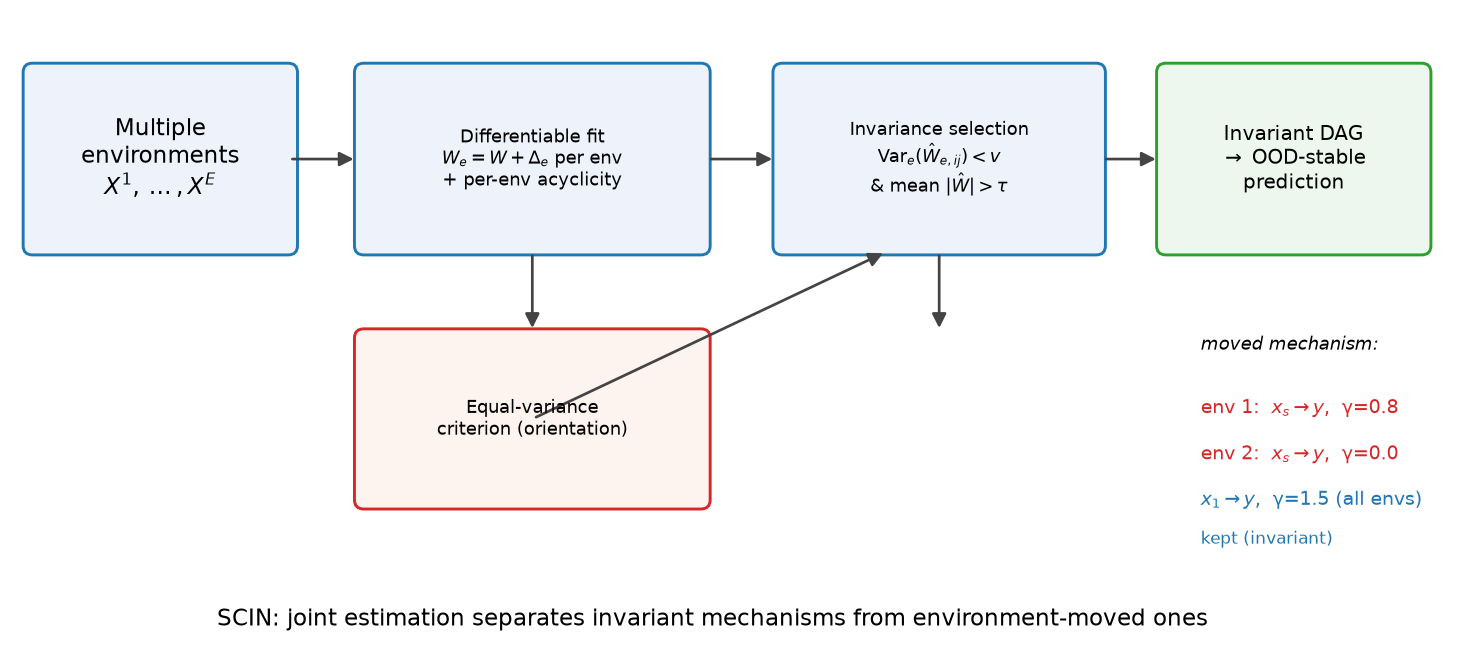
\includegraphics[width=0.9\textwidth]{results/figures/fig8_concept.png}
\caption{Concept schematic: environment-dependent mechanism moves around an invariant core; SCIN estimates the invariant set. (paper Fig. 1; file fig8_concept.png)}
\label{fig:fig8_concept}
\end{figure}

\begin{figure}[htbp]\centering
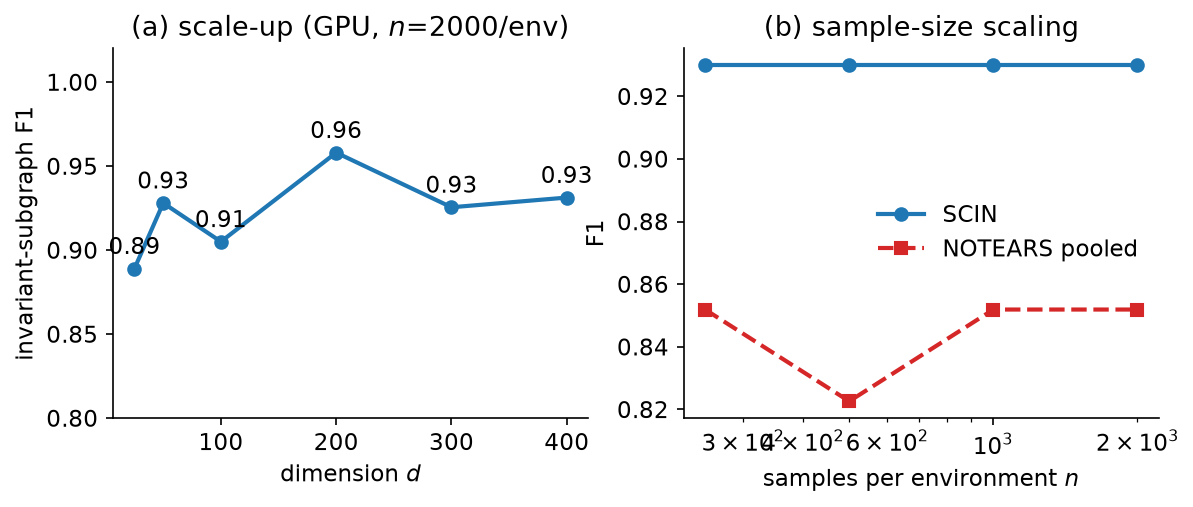
\includegraphics[width=0.9\textwidth]{results/figures/fig1_scaling.png}
\caption{Dimension scaling on GPU: directed F1 and precision at $d=25..400$ (RTX PRO 6000 Blackwell, fp64). (paper Fig. 2; file fig1_scaling.png)}
\label{fig:fig1_scaling}
\end{figure}

\begin{figure}[htbp]\centering
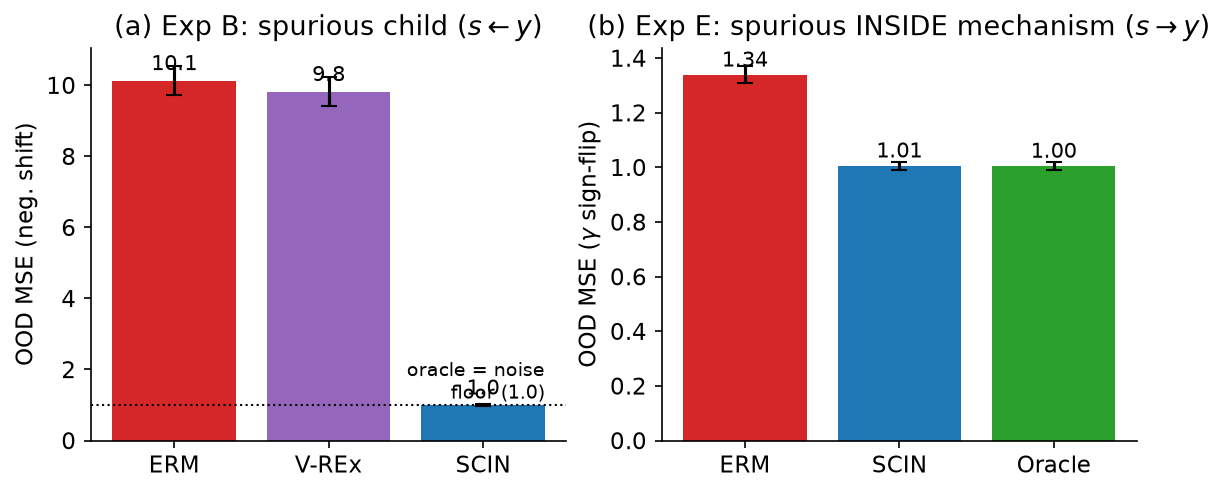
\includegraphics[width=0.9\textwidth]{results/figures/fig3_ood_bars.png}
\caption{OOD error under spurious shift: SCIN matches the oracle; ERM and V-REx pay the spurious term (Exp B, Exp E). (paper Fig. 3; file fig3_ood_bars.png)}
\label{fig:fig3_ood_bars}
\end{figure}

\begin{figure}[htbp]\centering
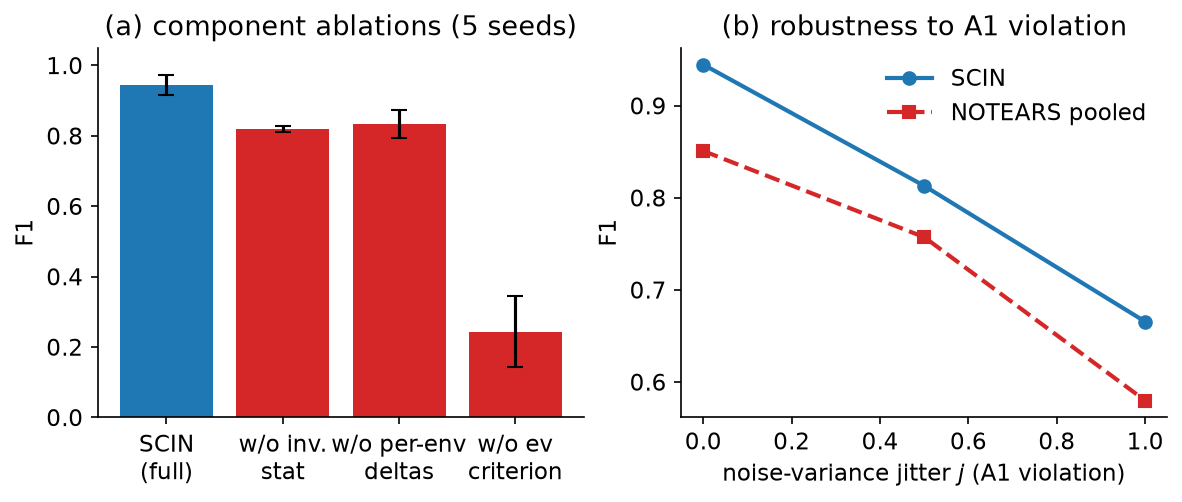
\includegraphics[width=0.9\textwidth]{results/figures/fig4_ablation_violation.png}
\caption{Ablation hierarchy (a) and A1-violation robustness (b). (paper Fig. 4; file fig4_ablation_violation.png)}
\label{fig:fig4_ablation_violation}
\end{figure}

\begin{figure}[htbp]\centering
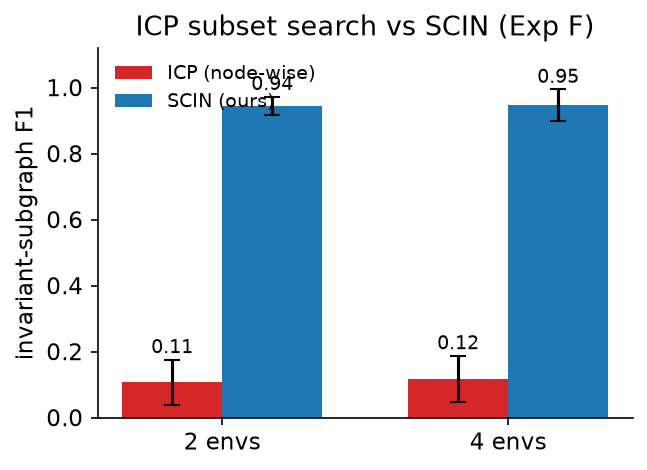
\includegraphics[width=0.9\textwidth]{results/figures/fig5_icp.png}
\caption{Node-wise ICP power collapse vs SCIN (Exp F). (paper Fig. 5; file fig5_icp.png)}
\label{fig:fig5_icp}
\end{figure}

\begin{figure}[htbp]\centering
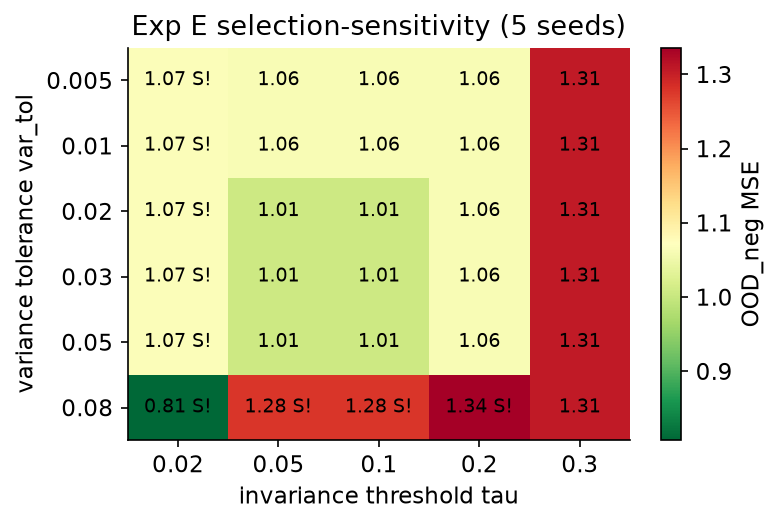
\includegraphics[width=0.9\textwidth]{results/figures/fig6_e_sens.png}
\caption{Selection-sensitivity plateau, var_tol x tau (Exp E). (paper Fig. 6; file fig6_e_sens.png)}
\label{fig:fig6_e_sens}
\end{figure}

\begin{figure}[htbp]\centering
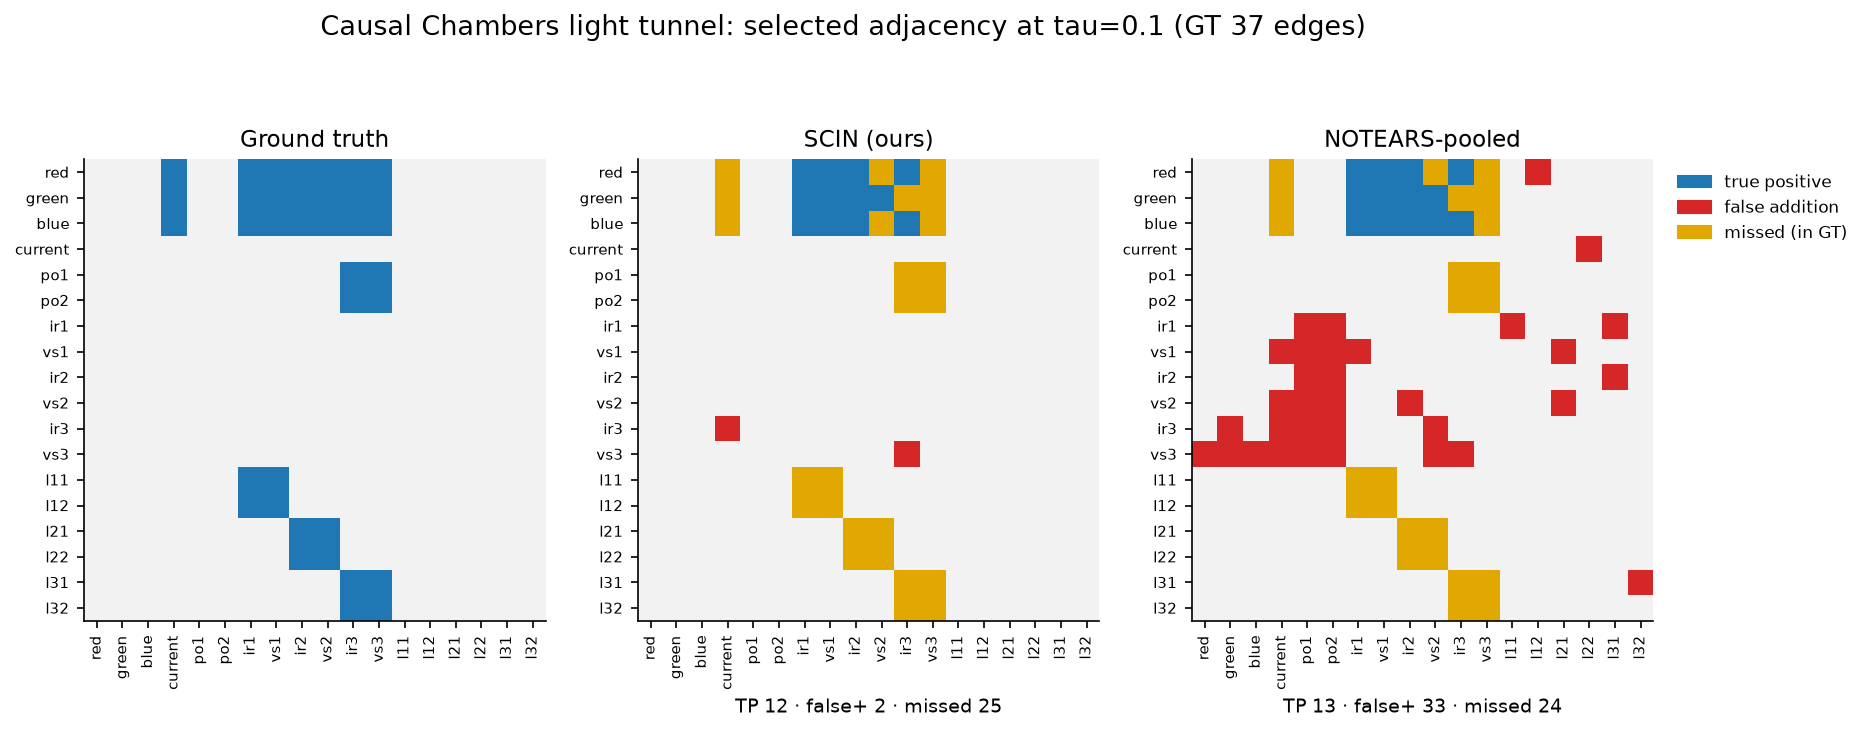
\includegraphics[width=0.9\textwidth]{results/figures/fig7_chambers_adjacency.png}
\caption{Causal Chambers: ground-truth vs SCIN vs pooled adjacency (18 nodes, seed 0). (paper Fig. 7; file fig7_chambers_adjacency.png)}
\label{fig:fig7_chambers_adjacency}
\end{figure}

\begin{figure}[htbp]\centering
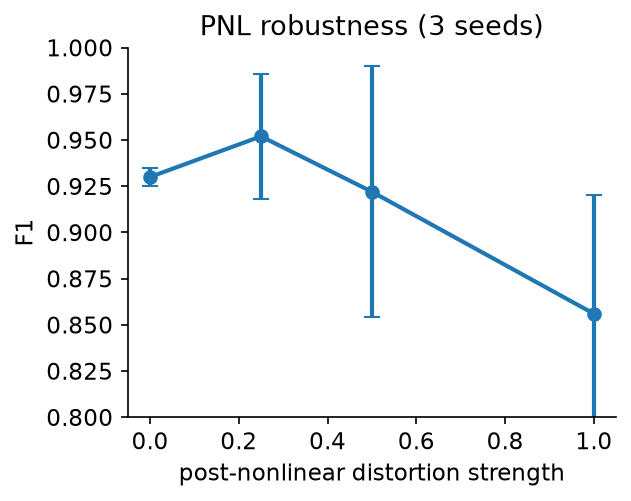
\includegraphics[width=0.9\textwidth]{results/figures/fig2_pnl.png}
\caption{Post-nonlinear robustness: F1 vs distortion strength. (paper Fig. 8; file fig2_pnl.png)}
\label{fig:fig2_pnl}
\end{figure}

\begin{figure}[htbp]\centering
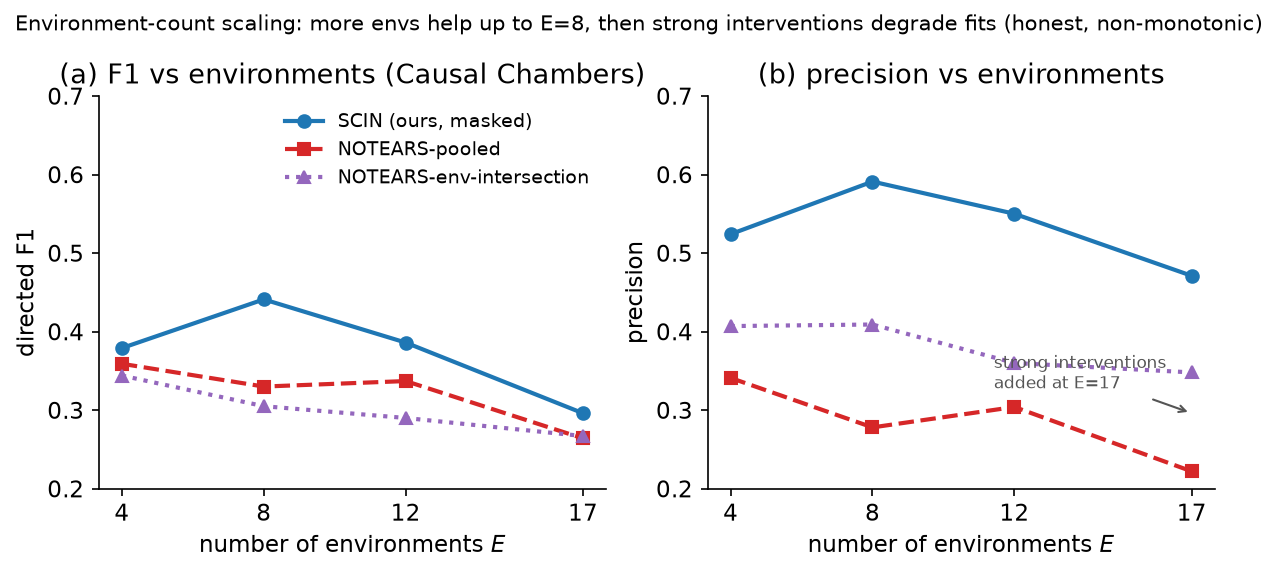
\includegraphics[width=0.9\textwidth]{results/figures/fig9_e_scaling.png}
\caption{Environment-count ladder on chambers ($E=4..17$). (paper Fig. 9; file fig9_e_scaling.png)}
\label{fig:fig9_e_scaling}
\end{figure}

\begin{figure}[htbp]\centering
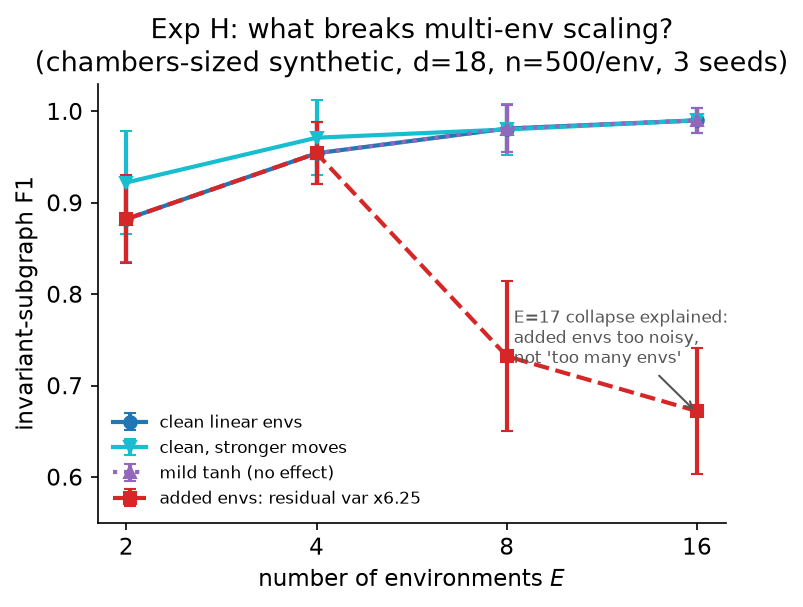
\includegraphics[width=0.9\textwidth]{results/figures/fig10_exp_h.png}
\caption{Experiment H: controlled env-ladder regimes. (paper Fig. 10; file fig10_exp_h.png)}
\label{fig:fig10_exp_h}
\end{figure}

\begin{figure}[htbp]\centering
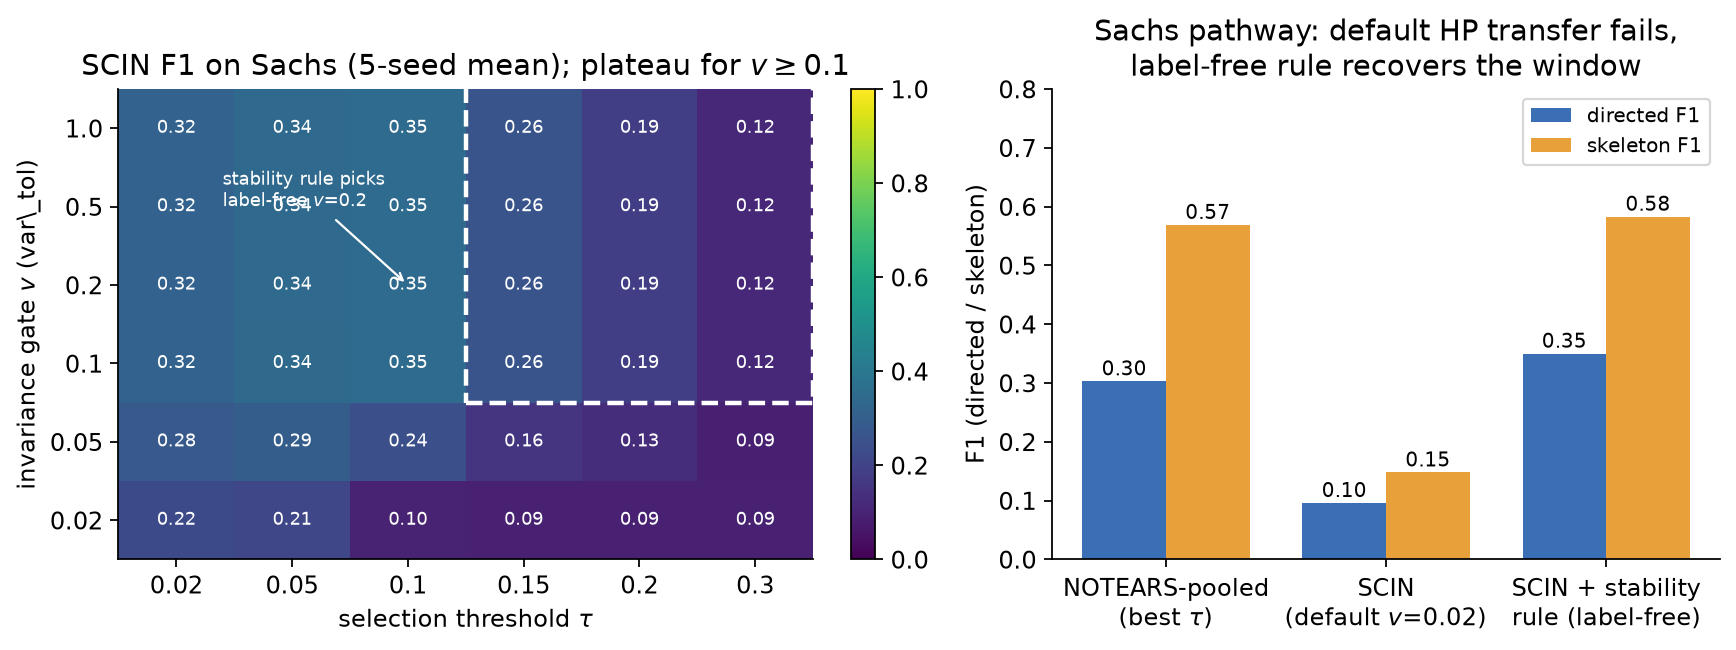
\includegraphics[width=0.9\textwidth]{results/figures/fig11_sachs.png}
\caption{Sachs domain pilot: sensitivity grid and label-free stability rule. (paper Fig. 11; file fig11_sachs.png)}
\label{fig:fig11_sachs}
\end{figure}


\end{document}
